\documentclass[12pt,oneside]{fithesis2}

\usepackage[english]{babel}       % Multilingual support
\usepackage[utf8]{inputenc}       % UTF-8 encoding
\usepackage[T1]{fontenc}          % T1 font encoding
\usepackage{hyperref}             % Clickable links
\usepackage{xcolor}               % For specifying the link colors
\usepackage{ccicons}              % https://ctan.org/pkg/ccicons
\usepackage{etoolbox}             % https://ctan.org/pkg/etoolbox
\usepackage{amsmath}              % https://ctan.org/pkg/amsmath
\usepackage{algorithm}            % https://ctan.org/pkg/algorithms
\usepackage{algpseudocode}        % https://ctan.org/pkg/algorithmicx
\usepackage{graphicx}             % https://ctan.org/pkg/graphicx

\hypersetup{
  plainpages = false,             % We have multiple page numberings
  %pdfpagelabels,                 % (alreaty set) Generate pdf page labels
  colorlinks,                     % We want nice colored links, not those ugly boxes
  linkcolor={red!50!black},
  citecolor={green!50!black},
  urlcolor={blue!80!black}
}

\thesislang{en}                   % The language of the thesis
\thesistitle                      % The title of the thesis
{Key derivation functions and their GPU implementation}
\thesissubtitle{Bachelor's Thesis}% The type of the thesis
\thesisstudent{Ondrej Mosnáček}   % Your name
\thesiswoman{false}               % Your gender
\thesisfaculty{fi}                % Your faculty
\thesisyear{Spring \the\year}     % The academic term of your thesis defense
\thesisadvisor{Ing. Milan Brož}   % Your advisor

\widowpenalty=500
\clubpenalty=500

\hyphenation{po-si-tive}

\begin{document}
  \FrontMatter                    % The front matter
    \ThesisTitlePage                % The title page
    
    % The license:
    This work is licensed under a \href{https://creativecommons.org/licenses/by-nc-sa/4.0/}{Creative Commons Attribution-NonCommercial-ShareAlike 4.0 International License}.
    \begin{center}
      \Large \ccbyncsa
    \end{center}
    
    \begin{ThesisDeclaration}       % The declaration
      \DeclarationText
      \AdvisorName
    \end{ThesisDeclaration}
    
    \begin{ThesisThanks}            % The acknowledgements (optional)
      \sloppy
      I would like to thank my supervisor for his guidance and support, and also for his extensive contributions to the Cryptsetup open-source project.
      
      Next, I would like to thank my family for their support and patience and also to my friends who were falling behind schedule just like me and thus helped me not to panic.
      
      \sloppy
      Last but not least, access to computing and storage facilities owned by parties and projects contributing to the National Grid Infrastructure MetaCentrum, provided under the programme “Projects of Large Infrastructure for Research, Development, and Innovations” (LM2010005), is also greatly appreciated.
    \end{ThesisThanks}
    
    \begin{ThesisAbstract}          % The abstract
      TODO
    \end{ThesisAbstract}
    
    \begin{ThesisKeyWords}          % The keywords
      key derivation function, PBKDF2, GPU, OpenCL, CUDA, password hashing, disk encryption, password cracking, LUKS
    \end{ThesisKeyWords}
    
    \tableofcontents                % The table of contents
%   \listoftables                   % The list of tables (optional)
%   \listoffigures                  % The list of figures (optional)
  
  \MainMatter                     % The main matter
    \chapter{Introduction}          % Chapters
      Encryption is the process of encoding information or data in such a way that only authorized parties can read it \cite{appliedCrypto, foundations}. The encryption uses a parameter -- the key. The key is an information that is only known to the authorized parties and which is necessary to read the encrypted data. In general, any piece of information can be used as the key, but since it usually has to be memorized by a human, it often has the form of a password or passphrase.
    
      Passwords and passphrases generally have the form of text (a variable-length sequence of characters), while most encryption algorithms expect a key in binary form (a long, usually fixed-size, sequence of bits or bytes). This means that for any password- or pass\-phrase-based cryptosystem it is necessary to define the process of converting the password (passphrase) into binary form. Merely encoding the text using a common character encoding (e. g. ASCII or UTF-8) and padding it with zeroes is often not sufficient, because the resulting key might be susceptible to various attacks. An \emph{attack} on a cryptographic key is an attempt by an unauthorized party to determine the key from publicly known information or from a certain partial information about the key (e. g. some knowledge about the domain from which the key was chosen, the first few bits of the key, etc.)."
    
      For this reason, a cryptographic primitive called \emph{key derivation function} (KDF, plural KDFs) is used to derive encryption keys from passwords. KDFs are also often used for \emph{password hashing} (transforming the password to a hash in such a way that it is easy to verify a given password against a hash, but infeasible to determine the original password from the hash) or \emph{key diversification} (also \emph{key separation}; deriving multiple keys from a master key so that it is infeasible to determine the master key or any other derived key from one or more derived keys) \cite{wiki:KDF, nist:sp800:108}.
    
      KDFs usually have various security parameters, such as the number of iterations of an internal algorithm, which control the amount of time or memory required to perform the derivation in order to thwart brute-force attacks. Another common parameter is the cryptographic salt, which is a unique or random piece of data that is used together with the password to derive the key. Its main purpose is to protect against dictionary and rainbow table attacks and it is usually not kept secret \cite{rfc2898}.
      
      \sloppy
      One possible application of KDFs is key derivation from passwords in disk encryption software. Disk encryption software encrypts the contents of a storage device (such as a hard disk or a USB drive) or its part (a disk volume or \emph{partition}) so that the data stored on the device can only be unlocked by one or more passwords or passphrases. The password/passphrase is entered when the user boots an operating system from the encrypted device or when they mount the encrypted partition to the filesystem.
      
      An example of a disk encryption program is \emph{cryptsetup}\footnote{\url{https://gitlab.com/cryptsetup/cryptsetup/wikis/home}} which uses the LUKS standard as its main format for on-disk data layout. In version 1 LUKS uses PBKDF2 as the only KDF for deriving encryption keys from passwords \cite{luks}. However, PBKDF2 has a range of weaknesses, one of them being high susceptibility to brute-force and dictionary attacks using GPUs\footnote{GPU = Graphics Processing Unit}, as this thesis aims to demonstrate.
    
      \section{Goals}
      The goal of this work is to compare the speed of a brute-force attack on a specific key derivation function (PBKDF2) performed on standard computer processors against an attack using GPUs.
      
      Modern GPUs can be programmed using various high-level APIs (such as OpenCL\footnote{\url{https://www.khronos.org/opencl/}}, CUDA\footnote{\url{http://www.nvidia.com/object/cuda_home_new.html}}, DirectCompute or C++ AMP) and can be used not only for graphics processing but also for general purpose computation. Due to their specific architecture GPUs are suitable for parallel processing of massive amounts of data. Tasks that can be split into many small subtasks which can be run in parallel can be processed by a single GPU several times faster than by a single CPU. As was shown by Harrison and Waldron \cite{Harrison}, using GPUs it is possible to accelerate also various algorithms of symmetric cryptography.
    
      This work also includes analysis of susceptibility of PBKDF2 to attacks using GPUs and the implementation of an illustration program performing a brute-force attack on the password of a LUKS\footnote{LUKS = Linux Unified Key Setup} encrypted partition.
    
      \section{Summary of results}
      TODO
      
      \section{Chapter contents}
      TODO
    
    \chapter{Key derivation functions}
      Key derivation functions are cryptographic primitives that are used to derive encryption keys from a secret value. Depending on the application, the secret value can be another key or a password or passphrase \cite{wiki:KDF}. A KDF that is designed for deriving cryptographic key from another key is called a \emph{key-based key derivation function} (KBKDF); a KDF that is designed to take a password or passphrase as input is called a \emph{password-based key derivation function} (PBKDF).
      
      \section{Key-based key derivation functions}
      Key-based key derivation functions are most often used to derive additional keys from a key that already has the properties of a cryptographic key -- that is, it is a truly random or pseudorandom binary string that is computationally indistinguishable from one selected uniformly at random from the set of all binary strings of the same length \cite{nist:sp800:108}.
      
      Since the input to a KBKDF is already a cryptographic key, KBKDFs usually do not try to make brute-forcing more difficult by making the algorithm more computationally complex. A good cryptographic key has entropy of at least 128 bits, which means there are at least $2^{128}$ possible keys. Testing so many keys would be infeasible even with a very fast algorithm and an enormous computer cluster.
      
      An example of a simple KBKDF is HKDF (HMAC-based extract-and-expand Key Derivation Function), which proceeds in two stages. The optional \emph{extract} stage first extracts a suitable pseudorandom key from the (possibly low-entropy) input key material and an optional salt. Then the \emph{expand} stage expands the extracted pseudorandom key, along with an optional context and application specific information (this can be used for key diversification), to the output key of the desired length \cite{hkdf, rfc5869}.
      
      \section{Password-based key derivation functions}\label{s:PBKDFs}
      As opposed to key-based key derivation functions, password-based key derivation functions are designed specifically to take low-entropy input such as a password or passphrase and to resist brute-force and dictionary attacks.
      
      \paragraph*{}
      A \emph{brute-force attack} is a kind of cryptanalytic attack in which the attacker attempts to determine a cryptographic key or password by systematically verifying (testing) all possible keys (this is also referred to as \emph{exhaustive key search}) \cite{appliedCrypto} or a large portion of all possible keys. In order to be able to perform the attack, the attacker must have a means to verify an unlimited number of different keys.
      
      A \emph{dictionary attack} is a kind of cryptanalytic attack in which the attacker attempts to determine a password by going through all passwords from a list of common passwords and/or (variations of) words from a dictionary \cite{appliedCrypto}. Dictionary attacks tend to be very successful in practice thanks to the users' tendency to pick very simple and predictable passwords.
      
      When the attacker tests the keys against a live system, the attack is called an \emph{online attack}. When the attacker holds an information sufficient to verify the keys on their own (for example one or more encryption plaintext and cryptotext pairs or password hashes), they can perform an \emph{offline attack} \cite{appliedCrypto}. An offline attack is usually significantly faster than an online attack because the attacker can optimize the verification algorithm and/or use specific hardware to accelerate the verification.
      
      \paragraph*{}
      PBKDFs aim to reduce the feasibility of these attacks by increasing the amount of time and/or memory required to test a single key. The basic principle of this approach is that in practice, the extra time/memory requirements are only a minor inconvenience for a user (especially given that these measures provide an increased resistance against a mass attack), while for an attacker (who has to repeatedly process millions or billions of possible passwords) this means that the resources needed to perform a brute-force (or dictionary) attack increase significantly.
      
      A well-designed PBKDF also takes into account the difference between the hardware that is used in the legitimate scenario and the hardware that the attacker might have available. A highly motivated and well-funded attacker might have access to massive amounts of computing power, might often be willing to wait even years until the password is found and might possess an expensive specialized hardware which would minimize the time and resources needed to successfully break the password. A typical user, on the other hand, will use a consumer-grade hardware (such as a personal computer or a laptop), so the PBKDF should be designed so that it performs with reasonable efficiency on the user's hardware, but at the same time it is difficult to utilize specialized hardware to gain advantage in an attack \cite{openwall:pwHashing}.
      
      In order to protect against attacks using highly parallel architectures, modern PBKDFs use \emph{sequential memory-hard functions}, which are designed in such a way that any time-efficient computation needs to use a certain configurable amount of memory (for a formal definition see \cite[chapter 4]{scrypt}). Requiring a certain non-trivial amount of memory to compute a single instance of the PBKDF increases the size of each compute unit, thus making any increase in parallelism more expensive (as opposed to functions that use only a small constant amount of memory) \cite{scrypt}.
      
      Another desirable property of PBKDFs is the ability to upgrade an existing derived key/hash to another having different (stronger) security parameters (e. g. the iteration count) without knowledge of the original password \cite{openwall:pwHashing}. However, there are no PBKDFs having this property currently available.
      % TODO: ?auth servers
      
      \paragraph*{}
      The most widely used password-based key derivation functions are currently \emph{PBKDF2} and \emph{bcrypt}.
      
      PBKDF2 was standardized under PKCS\footnote{PKCS = Public-Key Cryptography Standards; a group of standards published by RSA Security, Inc. (see \url{https://www.emc.com/emc-plus/rsa-labs/standards-initiatives/public-key-cryptography-standards.htm})} \#5, Version 2.0 in 1999 (also published as RFC 2898 in 2000 \cite{rfc2898}) and later specified in NIST Special Publication 800-132 \cite{nist:sp800:132} as the only password-based key derivation function approved by the U.S. National Institute of Standards and Technology. PBKDF2 is widely employed in many practical applications, such as Wi-Fi Protected Access (security protocols used to secure wireless networks), disk encryption software (Cryptsetup, TrueCrypt/VeraCrypt\footnote{\url{https://veracrypt.codeplex.com/}}, ...) and password managers (LastPass\footnote{\url{https://lastpass.com/}}, 1Password\footnote{\url{https://agilebits.com/onepassword}}, ...).
      
      Bcrypt was introduced in 1999 \cite{bcrypt} and although it incorporates several improvements over PBKDF2, it is not as widely used.
      
      In 2009, a new password-based key derivation function \emph{scrypt} was introduced \cite{scrypt}, which uses the aforementioned sequential memory-hard functions.
      
      \label{phc}
      In 2013, an open competition called \emph{Password Hashing Competition} was announced. The competition aims to ``identify new password hashing schemes in order to improve on the state-of-the-art'' \cite{phc}. The competition is organized by a group of cryptography experts, not by a standardization body. It is expected, however, that it will lead to a new standard for password-based key derivation and password hashing.
      
      \section{PBKDF2}\label{s:PBKDF2}
      PBKDF2 is a generic password-based key derivation function -- its definition depends on the choice of an underlying pseudorandom function (PRF). The specification \cite{rfc2898} does not impose any additional constraints on the PRF, other than that it takes two arbitrarily long octet strings as input and outputs an octet string of a certain fixed length. In appendix B.1, the specification presents the HMAC message authentication code (HMAC; specified in RFC 2104 \cite{rfc2104}) using SHA-1 as the underlying hash function as an example for the PRF. The practical applications of PBKDF2 use HMAC (with various underlying hash algorithms) almost solely as the underlying PRF. The instantiations of PBKDF2 using specific PRFs are often denoted as PBKDF2-\emph{PRF}, where \emph{PRF} is the name of the PRF used (for example PBKDF2 using HMAC-SHA1 would be denoted as PBKDF2-HMAC-SHA1).
      
      PBKDF2 takes two important security parameters -- \emph{salt} and \emph{iteration count}.
      
      As noted in \cite[section 4.1]{rfc2898}, salt has two main purposes in password-based cryptography:
      \begin{enumerate}
        \item To make it infeasible for an attacker to precompute the results of all possible keys (or even the most likely ones), that is to prevent rainbow-table attacks (described in \ref{s:PBKDFs}). For example, if the salt is 64 bits long, a single input key (password) has $2^{64}$ possible derived keys, depending on the choice of salt.
        \item To make it unlikely that the same key will be derived twice. This is important for some encryption and authentication techniques.
      \end{enumerate}
      
      The iteration count represents the number of successive computations of the underlying PRF that are required to compute each block of the derived key. The purpose of the iteration count is to increase the time cost of the function, in order to mitigate brute-force and dictionary attacks, as discussed in \ref{s:PBKDFs}. The original specification recommends a minimum of 1000 iterations to be used \cite[section 4.2]{rfc2898}, however there are concerns that this number may not be sufficient and that it should be determined dynamically according to current technology \cite[chapter 7]{Durmuth} \cite[footnotes 7, 8]{luks}.
      
      \subsection{Description of the algorithm}
      Let $hLen$ be the length in octets of the output of the pseudorandom function \Call{PRF}{}. PBKDF2 with \Call{PRF}{} as the underlying function takes the following input parameters \cite{rfc2898}:
      \begin{itemize}
        \item $P$ -- the password (an octet string)
        \item $S$ -- the salt (an octet string)
        \item $c$ -- the iteration count (a positive integer)
        \item $dkLen$ -- the intended length in octets of the derived key (a positive integer, at most $(2^{32} - 1) \cdot hLen$)
      \end{itemize}
      
      The following pseudocode illustrates the process of computation of PBKDF2 with underlying function \Call{PRF}{}, as per RFC 2898 \cite{rfc2898}:
      \begin{algorithm}[H]
        \caption{PBKDF2}
        \begin{algorithmic}[1]
          \Function{PBKDF2}{$P, S, c, dkLen$}
            \If{$dkLen \le (2^{32} - 1) \cdot hLen$}
              \State output ``derived key too long'' and
         stop
            \EndIf
            \State $l \gets \lceil dkLen / hLen\rceil$ \Comment{{\footnotesize $l$ is the number of $hLen$-octet blocks in the derived key, rounding up}}
            \State $r \gets dkLen - (l - 1) \cdot hLen$ \Comment{{\footnotesize $r$ is the number of octets in the last block}}
            \For{$k \gets 1$, $l$}
              \State $T_k \gets \Call{PRF}{P, S \mid \operatorname{int}(k)}$
              \For{$i \gets 2$, $c$}
                \State $T_k \gets T_k \oplus \Call{PRF}{P, T_k}$
              \EndFor
            \EndFor
            \State \Return $T_1 \mid T_2 \mid ... \mid T_l[0..r - 1]$
          \EndFunction
        \end{algorithmic}
      \end{algorithm}
      
      Here, $A \mid B$ is the concatenation of octet strings $A$ and $B$; $\operatorname{int}(x)$ is a four-octet encoding of the integer $x$ with the most significant octet first (i. e. the big-endian encoding of the integer $x$); $A \oplus B$ is the bitwise exclusive disjunction (also called ``exclusive or'' or ``XOR'') of octet strings $A$ and $B$; $A[i..k]$ denotes an octet string produced by taking the $i$-th through the $k$-th octet of the octet string $A$.
      
      As follows from the algorithm, the derived key is divided into blocks of $hLen$ octets, each of which can be computed independently. Each of these output blocks is computed using the same algorithm, seeded by its one-based index, which allows for the blocks to be computed in parallel.
      
      The computation of each block is performed by applying $c$ iterations of the PRF to an initial seed consisting of the salt and a binary representation of the index of the block. After each iteration, the output from the PRF is combined with the result of the previous iteration using the bitwise XOR operation, in order to ``reduce concerns about the recursion degenerating into a small set of values'' \cite[section 5.2]{rfc2898}.
      
      \section{Scrypt}
      The scrypt key derivation function takes the following input parameters \cite[chapter 7]{scrypt}:
      \begin{itemize}
        \item $P$ -- the password (an octet string)
        \item $S$ -- the salt (an octet string)
        \item $N$ -- the CPU/memory cost parameter
        \item $r$ -- the block size parameter
        \item $p$ -- the ``parallelization'' parameter
        \item $dkLen$ -- the intended length in octets of the derived key
      \end{itemize}
      
      The $P$, $S$ and $dkLen$ parameters have the same meaning as in PBKDF2 described in the previous section (\ref{s:PBKDF2}). The remaining parameters can be tuned by the user according to the amount of computing power and memory available.

      Increasing (decreasing) the $N$ parameter linearly increases (decreases) both the amount of memory (space complexity) and the amount of computation power required to compute the KDF (time complexity), if the implementation makes full use of random access memory. Alternatively, the implementation may choose to use constant amount of memory, in which case the time complexity becomes $O(N^2)$ instead of $O(N)$ \cite[chapter 5, proof of theorem 1]{scrypt}. This allows for a time-memory trade-off, which can be exploited to gain better performance on GPUs \cite{scrypt:tradeoff, openwall:pwHashing}.
      
      Increasing (decreasing) the $r$ parameter also linearly (increases) time and space complexity, but does not allow for a similar time-memory trade-off. However, theoriginal scrypt paper recommends using only a small, relatively fixed value for $r$ (8) and suggests instead increasing the $N$ parameter (in the password cracking time estimates \cite[chapter 8]{scrypt} Percival uses values $N = 2^{14}$ or $2^{20}$ and $r = 8$).
      
      The $p$ parameter also has linear scaling effect on time and space complexity, but allows up to $p$ parallel processes/computation units to be used for computation (with the exception of the fast initial and final steps). The value for this parameter recommended by the scrypt specification is 1. However, the author notes that future advancement in technology might lead to higher values being more efficient \cite[chapter 7]{scrypt}.
      
      The time-memory trade-off problem was addressed in scrypt's successor, \emph{yescrypt}, which is one of the finalists of the Password Hashing Competition (see \ref{phc}).
      
      As opposed to PBKDF2, the pseudorandom function and hash function used internally in scrypt are strictly defined in the specification.
      
    %\chapter{Attacks on key derivation functions}
    \chapter{Acceleration of algorithms using GPUs}
      Originally designed for acceleration of computer graphics, GPUs have recently also become a powerful platform for general-purpose parallel processing. The fast-growing computer game industry has motivated a rapid advancement of graphics hardware, which is gradually outperforming general-purpose CPUs by several orders of magnitude.
      
      To be able to optimally use the computational potential of GPUs, the task being computed must have certain properties. The task must be divisible into multiple small tasks that all perform the same computation over different pieces of data. Each of these tasks must only require a very small amount of memory.
      
      In the following section, we describe the architecture of GPUs in detail and discuss the considerations for implementing algorithms on these devices.
      
      \section{GPU architecture}
      A standard, general-purpose CPU consists of a single and relatively complex \emph{control unit} (CU)\footnote{The CU is the part of the CPU that decodes a program's instructions and controls the operation of the rest of the CPU, the computer's memory and the input/output devices based on these instructions \cite{wiki:CU}.} and one or more \emph{arithmetic logic units} (ALU)\footnote{The ALU ``performs arithmetic and bitwise logical operations on integer binary numbers'' \cite{wiki:ALU}.}. Between the CPU and main memory there are several layers of cache -- a small and fast memory that stores recently accessed contents of the main memory for faster access.
      
      \paragraph*{}
      A GPU consists of several main parts -- multiple \emph{streaming multiprocessors}, the \emph{global memory}, the \emph{texture memory} and \emph{constant memory}.
      
      \begin{figure}
        \centering
        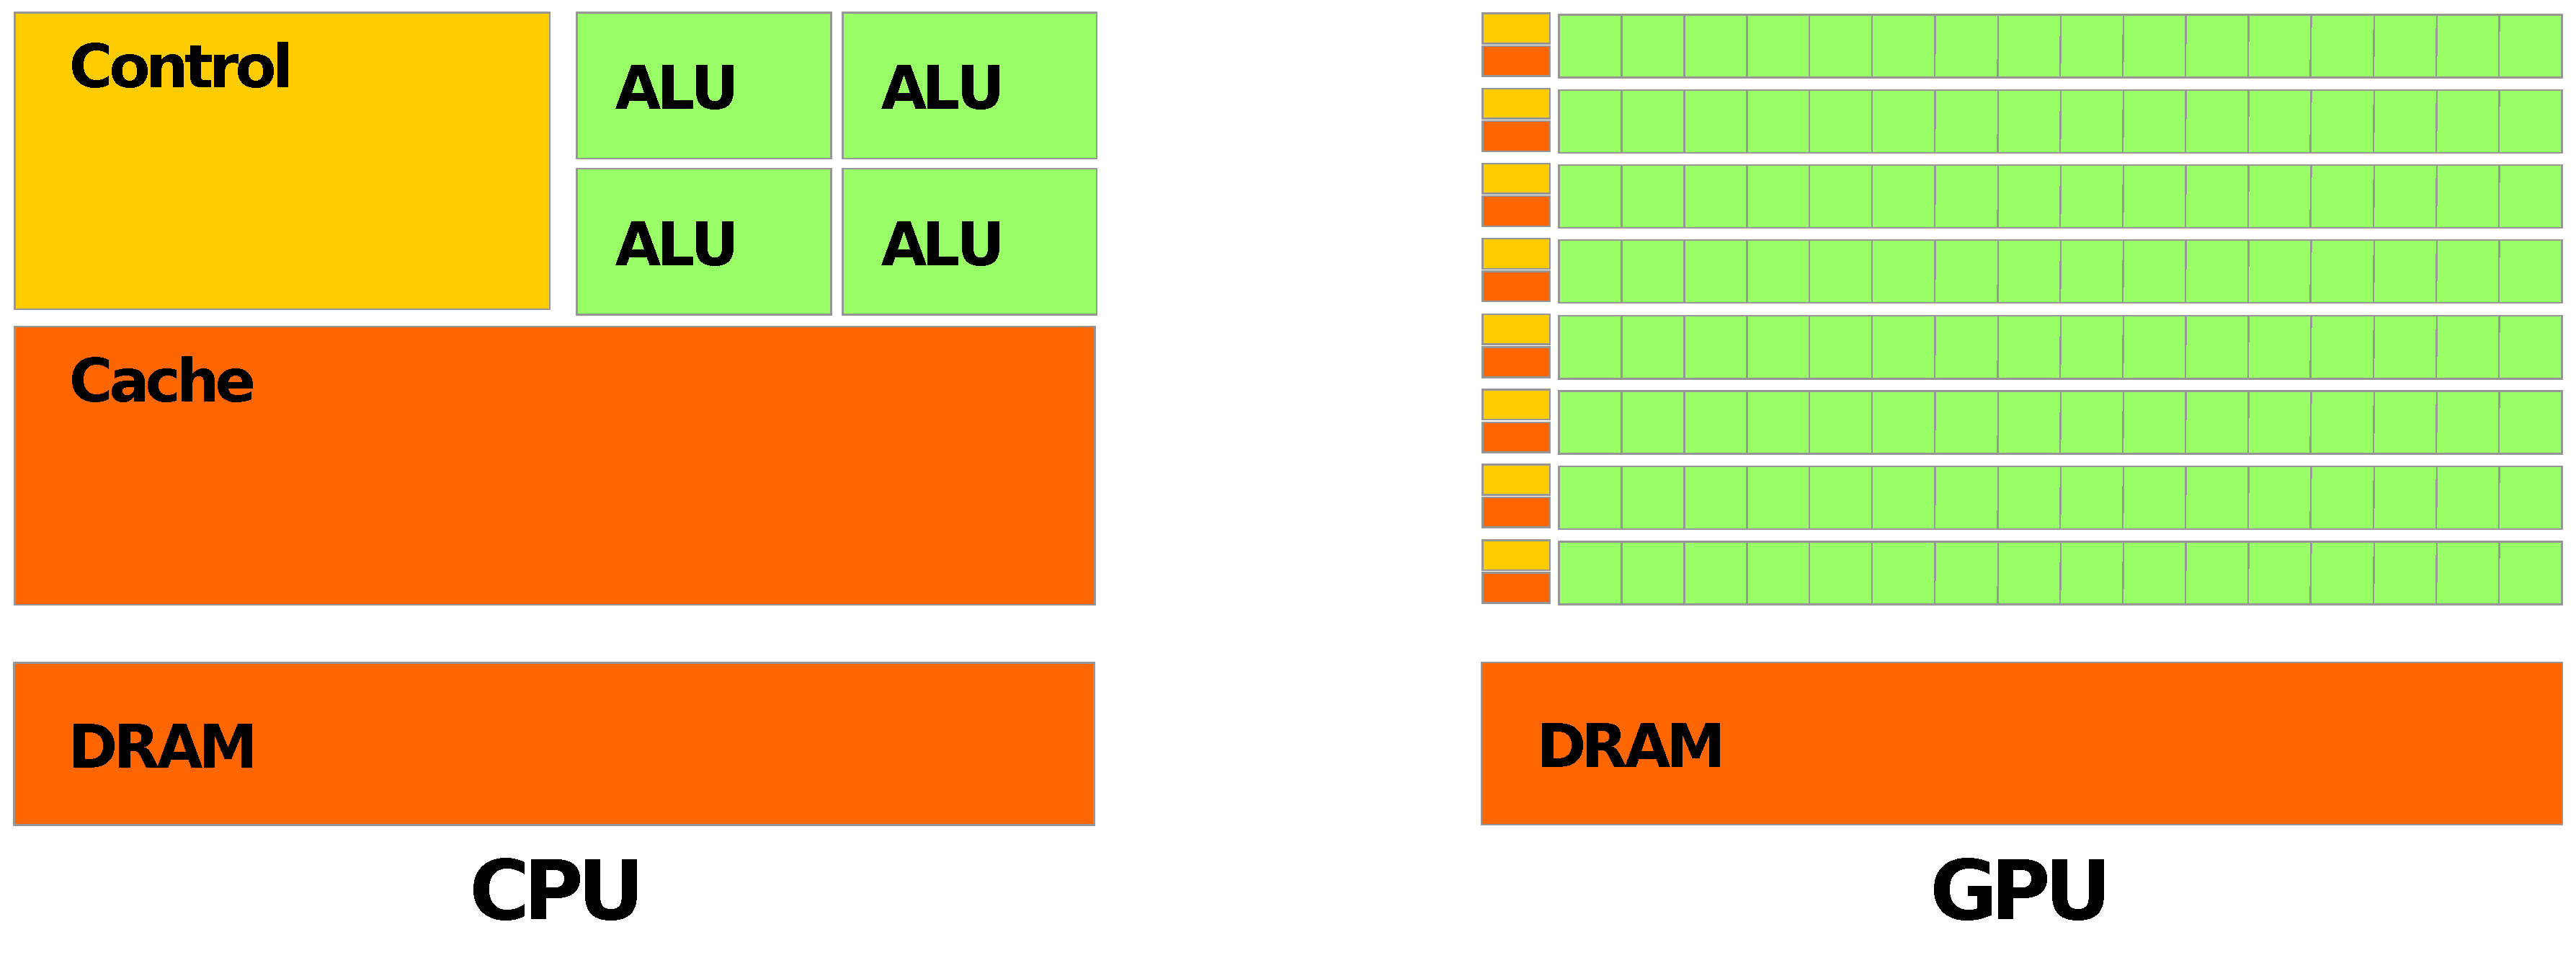
\includegraphics[width=\linewidth]{images/gpu-vs-cpu.eps}
        \caption{CPU vs GPU architecture\protect\footnotemark}
      \end{figure}
      
      Each streaming multiprocessor contains a single \emph{instruction unit} (equivalent to the CPU's control unit) with instruction cache, \emph{constant cache} (a cache for constant memory), \emph{shared memory} and several \emph{thread processors}. Each thread processor is capable of executing several groups (called \emph{warps}) of \emph{threads}. All threads in a warp execute the same program, which is called a \emph{kernel} \cite{nvidia:gpuArch}.
      
      \footnotetext{Copyright \textcopyright~2010, NVIDIA Corporation, published under a \href{https://creativecommons.org/licenses/by/3.0/}{Creative Commons Attribution 3.0 Unported License}; source: \url{https://commons.wikimedia.org/w/index.php?title=File:Cpu-gpu.svg&oldid=156649300}}
      
      Streaming multiprocessors are designed for \emph{data parallelism} -- threads should execute the same sequence of instructions over different data. Kernels may contain branches and loops -- in this case both paths of each branch are executed in each thread. Branches should, however, be used carefully -- if the threads diverge (that is, they end up executing different parts of the kernel) the computation becomes very inefficient. Thread scheduling is handled by hardware automatically, which minimizes scheduling overhead. As opposed to CPUs, SMs in GPUs always execute instructions in-order instead of out-of-order. Memory latency is avoided by temporarily switching to another thread while a memory transaction is in progress \cite{nvidia:gpuArch}.
      
      \begin{figure}
        \centering
        \includegraphics[width=\linewidth]{images/sm.png}
        \caption{Streaming multiprocessor}
      \end{figure}
      
      \subsection{Memory hierarchy}
      From ...
      
    \chapter{Implementing PBKDF2 on GPUs}
    \chapter{Comparison of CPU and GPU attack speeds}
    \chapter{Conclusion}
    
    \iffalse
    \appendix
    \chapter{First appendix}        % Appendices
      TODO
    \chapter{Another appendix}
      TODO
    \fi
    
    % Bibliography goes here
    % shut up those bibliography warnings:
    \apptocmd{\sloppy}{\hbadness 10000}{}{}
    
    \bibliographystyle{acm}
    \bibliography{thesis}
    
    % Index goes here (optional)
\end{document}
